 % % % % % % % % % % % % % % % % % % % % % % % % % % % % % % % % % % % %
 % % % % % % % % % % % % % % % % % % % % % % % % % % % % % % % % % % % %
 % % % % % % % % % % % % % % % % % % % % % % % % % % % % % % % % % % % %

\documentclass[paper=a4, fontsize=11pt]{scrartcl} 
\usepackage[T1]{fontenc} 
\usepackage[utf8]{inputenc}
\usepackage[english]{babel}
 
\usepackage[nottoc]{tocbibind}
\usepackage{fourier} 
\usepackage{float}
\usepackage{graphicx}
\usepackage[english]{babel} 
\usepackage{amsmath,amsfonts,amsthm} 
\usepackage{listings}
\usepackage{sectsty} 
\allsectionsfont{\centering \normalfont\scshape} 
\usepackage{fancyhdr} % Custom headers and footers
\usepackage{float}
\usepackage{courier}
\usepackage{parskip}
\usepackage{geometry}




 % % % % % % % % % % % % % % % % % % % % % % % % % % % % % % % % % % % %

\pagestyle{fancyplain} 
\fancyhead{} 
\fancyfoot[L]{} 
\fancyfoot[C]{} 
\fancyfoot[R]{\thepage} 
\renewcommand{\headrulewidth}{0pt} 
\renewcommand{\footrulewidth}{0pt} 
\setlength{\headheight}{13.6pt} 
\numberwithin{equation}{section} 
\numberwithin{figure}{section} 
\numberwithin{table}{section}
\setlength\parindent{0pt} 




 % % % % % % % % % % % % % % % % % % % % % % % % % % % % % % % % % % % %

\newcommand{\horrule}[1]{\rule{\linewidth}{#1}}  
 
 % % % % % % % % % % % % % % % % % % % % % % % % % % % % % % % % % % % %

\title{	
\normalfont \normalsize 
\textsc{Barcelona Graduate School of Economics - Data Science} \\ [25pt]
\horrule{2pt} \\[0.5cm] 
\huge Random Forest Cover Type Prediction  \\ 
\horrule{2pt} \\[0.5cm] 
}

\author{Jessica Leal \  \ \ \ Tim Kreienkamp \  \  \  \ Philipp Schmidt} 

\author{J\'essica Leal, Tim Kreienkamp and Philipp Schmidt} 
\date{}



 % % % % % % % % % % % % % % % % % % % % % % % % % % % % % % % % % % % %
\geometry{legalpaper, margin=1.3in}


\begin{document}



 % % % % % % % % % % % % % % % % % % % % % % % % % % % % % % % % % % % %


\maketitle


 % % % % % % % % % % % % % % % % % % % % % % % % % % % % % % % % % % % %



\section{Introduction}
\subsection{Dataset Characteristics}
In this project, we work with a training data set of 50,000 observations - with labels - and a testing set - without labels - of 100,000 observations. Our aim is to predict a seven-class variable in which each label is a different type of forest cover using cartographic variables. We have 10 numeric variables and 44 binary variables for qualitative aspects of the forest segment. The include information about fire, roads, hydrology, elevation and different soil types. 
A forest cover type is the pre-dominant type of tree that grows in a specific forest segment. 

 % % % % % % % % % % % % % % % % % % % % % % % % % % % % % % % % % % % %
\subsection{Establishing a Baseline}
We first establish a baseline, using the out of bag error untuned random Forest to give us an idea of how well a very simple model would do. This serves as a yardstick with which all more complex modeling are measured.
The out of bag error of this simple random forest is 0.25 and the test error is 0.8.

 % % % % % % % % % % % % % % % % % % % % % % % % % % % % % % % % % % % %

\section{Exploratory Analysis}

The exploratory analysis is conducted to develop a thorough understanding of the dataset, to find relationships between the features and suggest new variables that might help to predict forest cover type. Within this report we focus on relationships among features and the creation of new variables.

\subsection{Relation between features}
We use scatterplots to observe the relationships between the quantitative features.\\

\begin{figure}[H]
    \centering
    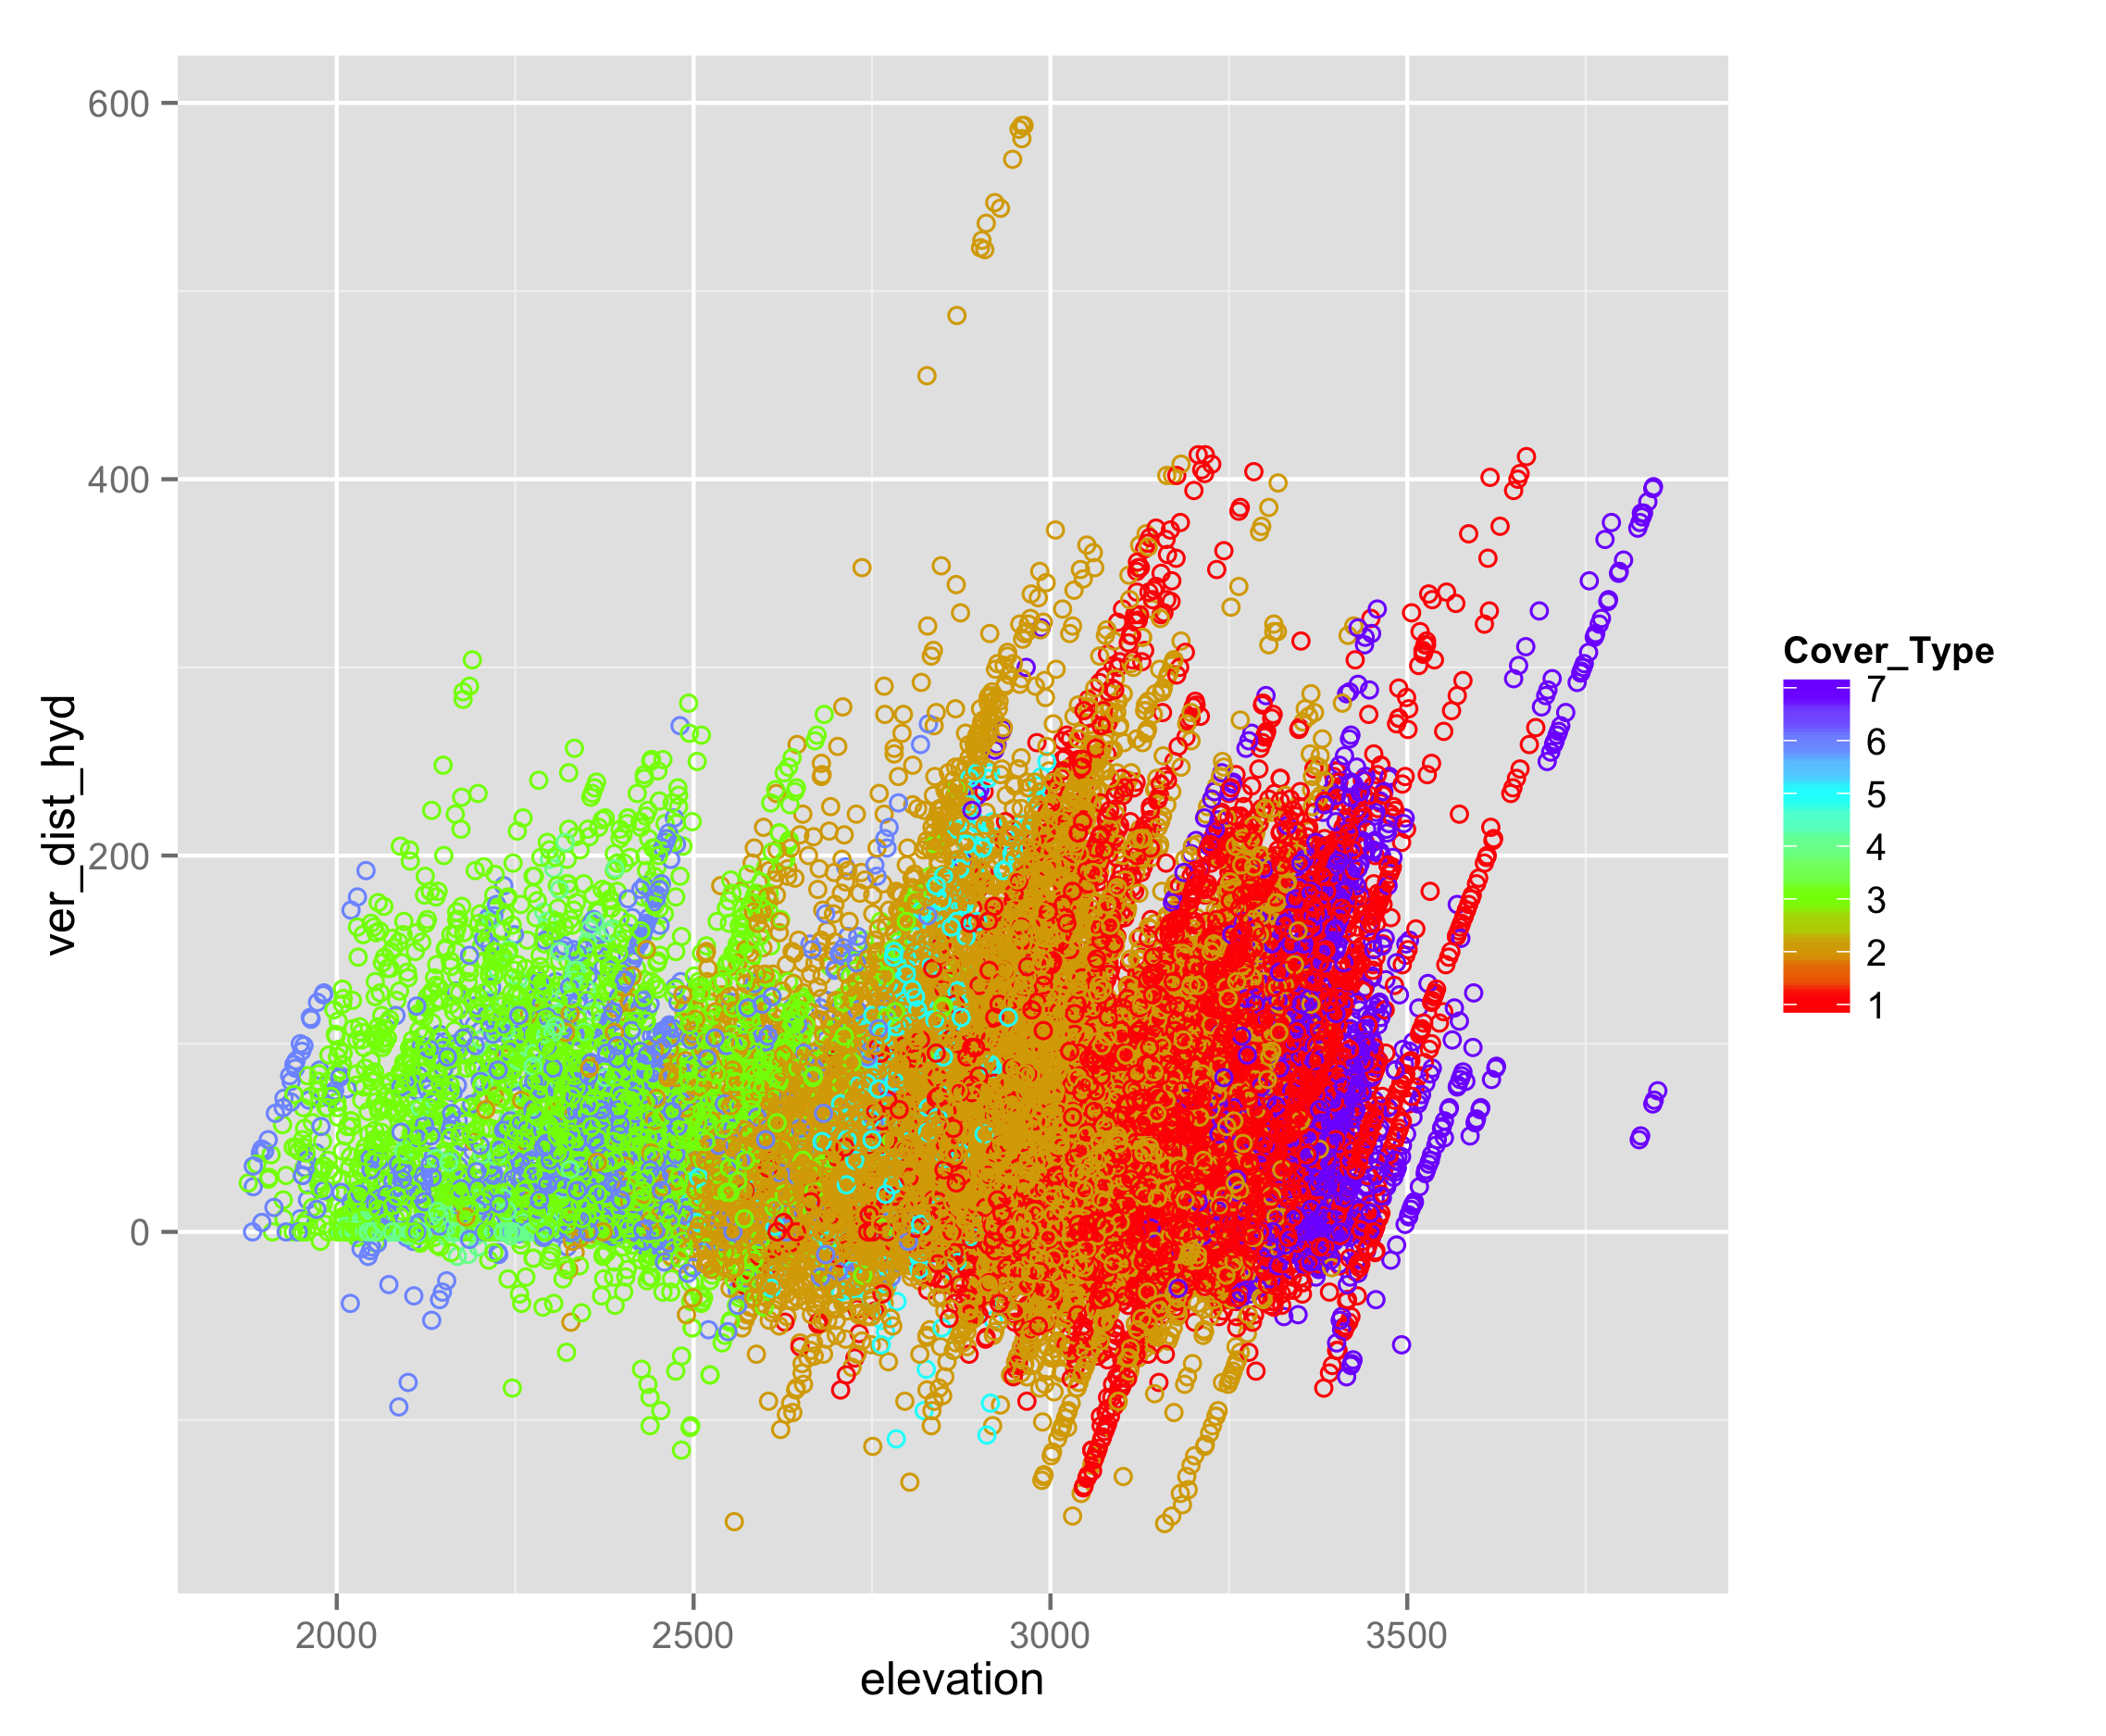
\includegraphics[width=0.8\textwidth]{elevation-ver_dist.png}
    \caption{Plotting elevation vs. \lstinline{vert_dist_hyd}}
    \label{fig:errors}
\end{figure}

There appears to be a strong relationship between the vertical distance and elevation within the groups. We thus create a new variable to account for this relationship which will later be tested for its predictive power. \\

\begin{lstlisting}
EVTH <-  data$elevation - data$ver_dist_hyd
\end{lstlisting}


\begin{figure}[H]
    \centering
    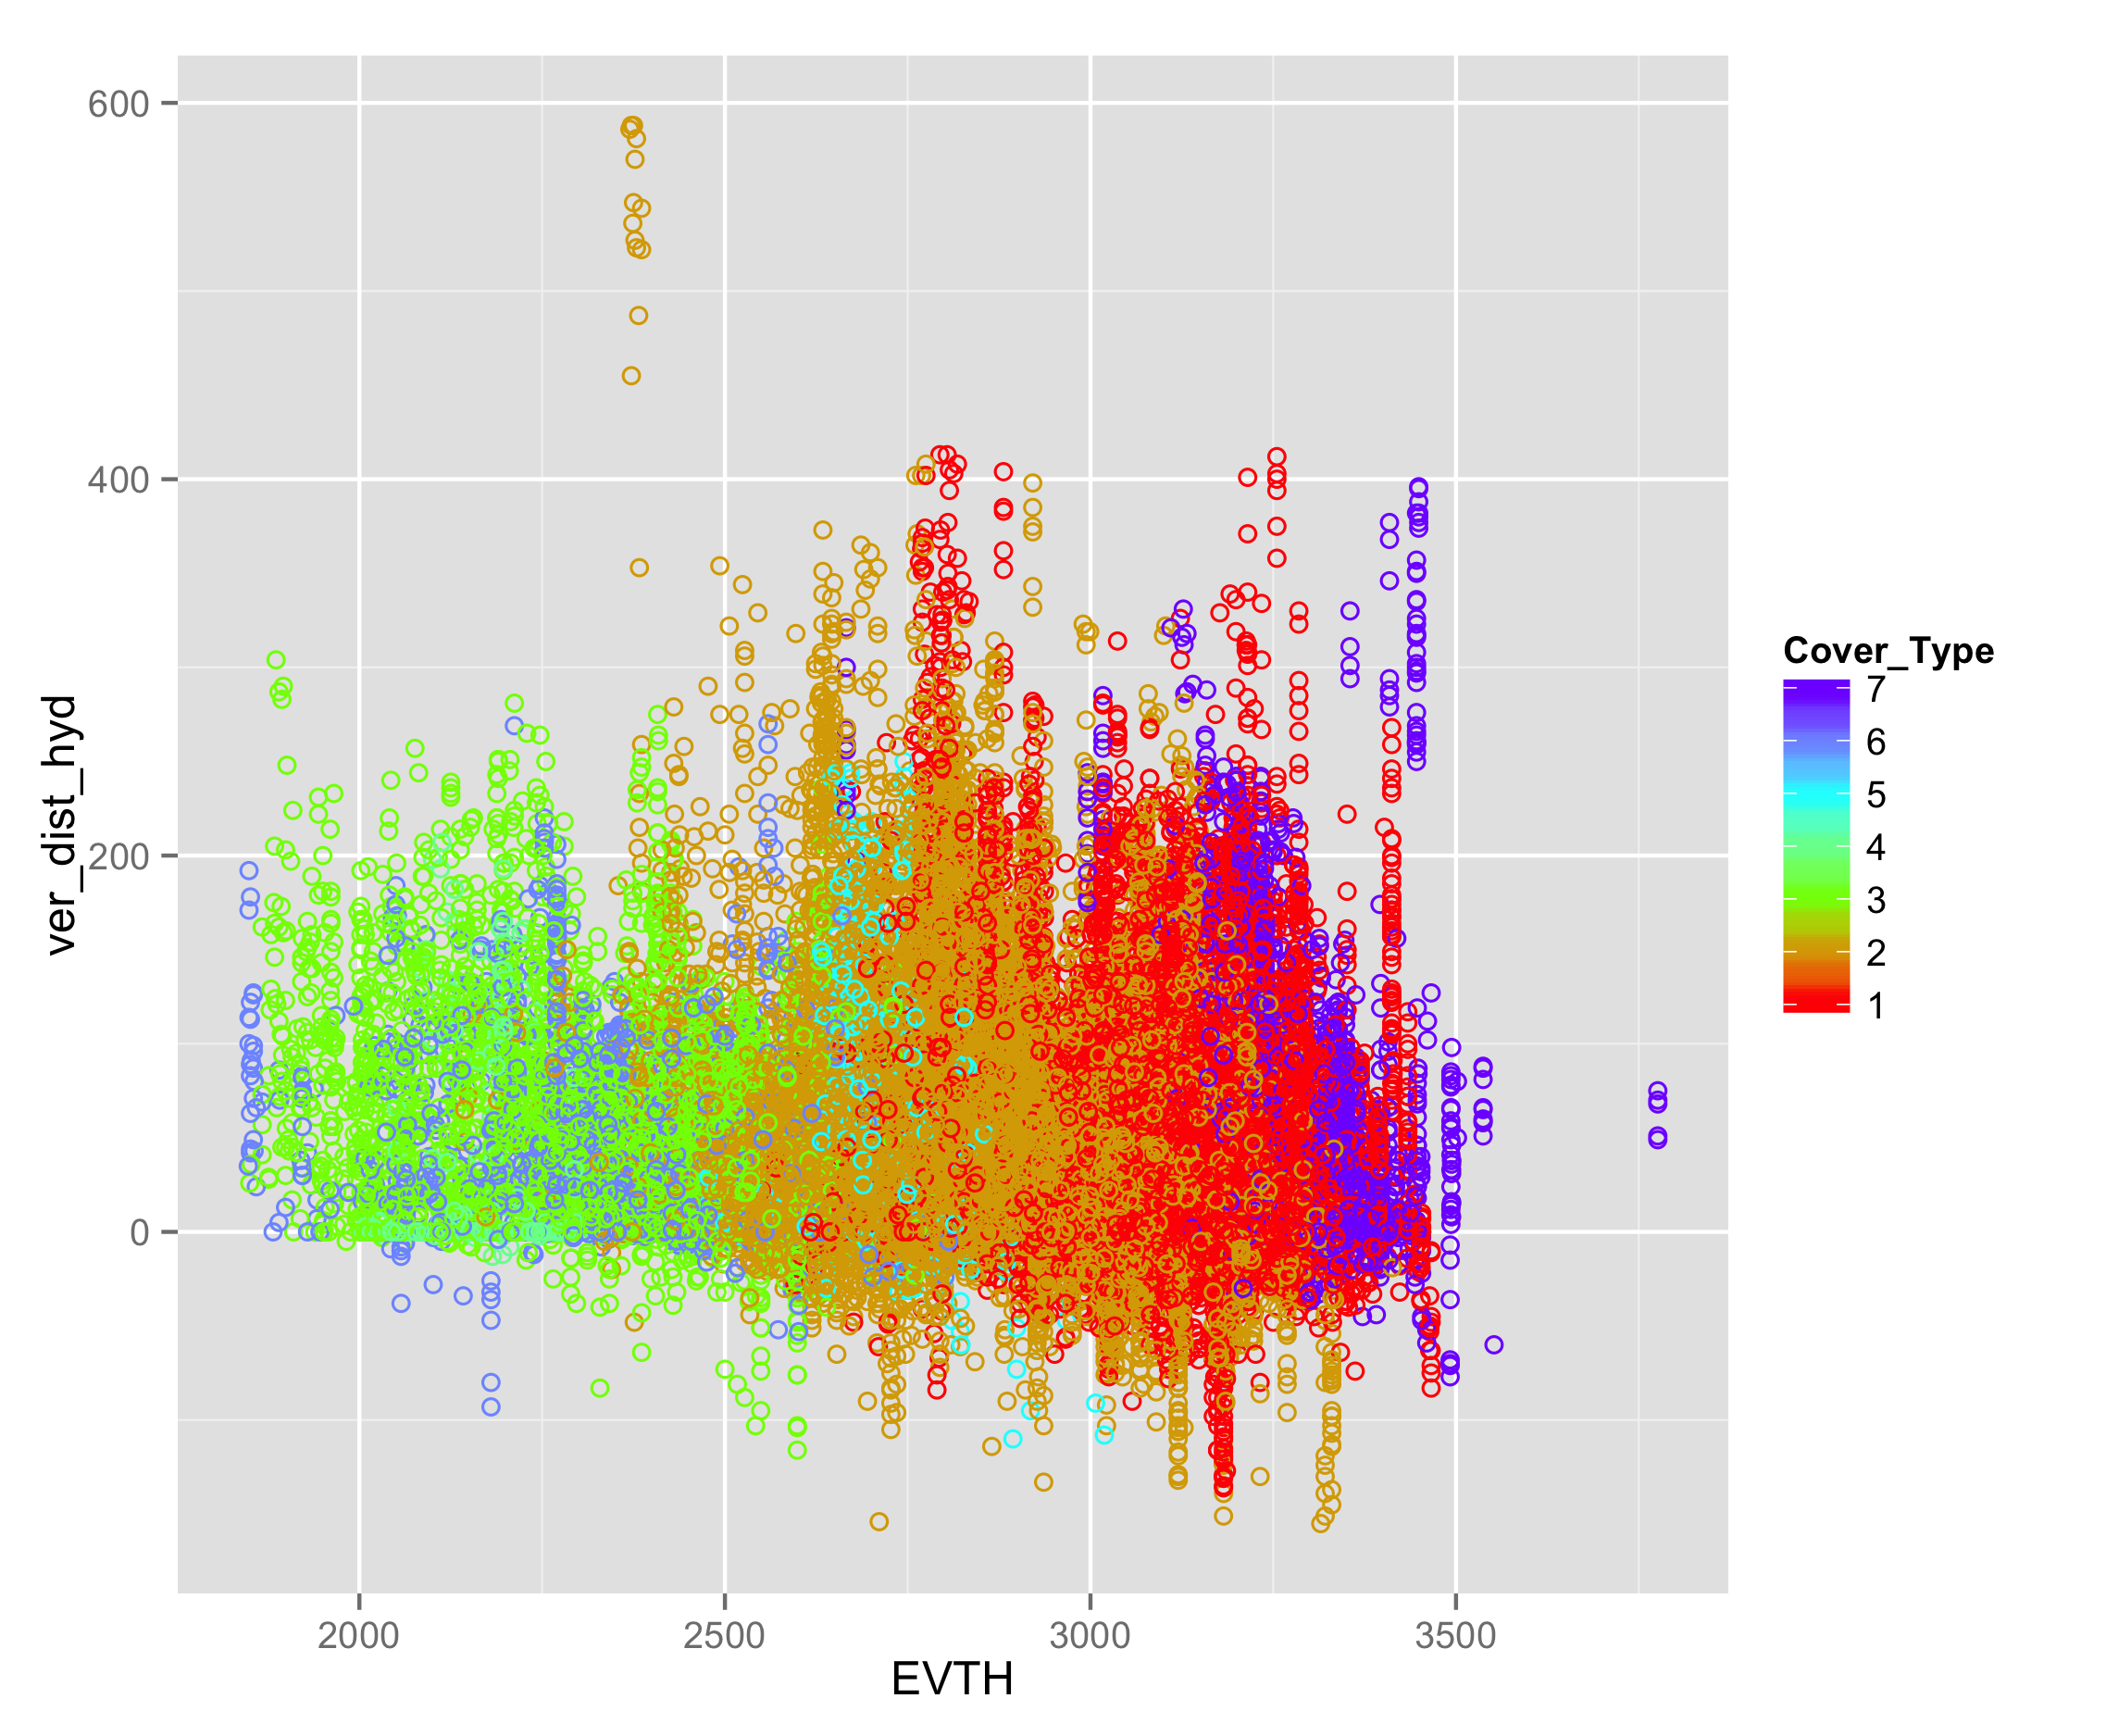
\includegraphics[width=0.8\textwidth]{EVTH-ver_dist.png}
    \caption{IEVTH vs. \lstinline{vert_dist_hyd}}
    \label{fig:errors}
\end{figure}

The created feature seems to separates the groups well. We observed a similar relationship between the horizontal distance and elevation and thus add the following variable.\\

\begin{lstlisting}
EDTH <- elevation - hor_dist_hyd*0.2
\end{lstlisting}

Using the same reasoning we observe and create the following variables.
\begin{lstlisting}
Hydro_Road_1 <- abs(hor_dist_hyd + hor_dist_road)
Fire_Road_1 <- abs(hor_dist_fire +hor_dist_road)
hydro_road_2 <-  abs(hor_dist_hyd - hor_dist_road)
Fire_Road_2 <- abs(hor_dist_fire - hor_dist_road)
\end{lstlisting}



 % % % % % % % % % % % % % % % % % % % % % % % % % % % % % % % % % % % %
\section{Methods}

\subsection{K-Nearest Neighbor}
With this method\footnote{Firstly proposed by Fix and Hodges (1951) \cite{knn}}, we try to classify each new observation in the test set taking into consideration the majority label from its the labels of its a certain number of nearest neighbors (K). In our case, we used the Euclidean distance as a measure of closeness between observations.

\subsection{Gradient Boosting  \& Random Forest}
Both gradient boosting and random forest are so-called ensemble based methods. They combine many models (weak learners) with little predictive power to form one powerful model. 
Gradient Boosting,  \footnote{First proposed by Friedmann 200, \cite{Friedman00greedyfunction}} builds an additive model by fitting regression trees in a stage-wise fashion to the gradient of a (convex, differentiable) loss function.
Random forest \footnote{Firstly proposed by Breiman, L. (2001) \cite{random} } tries to create a strong classifier from the weighted sum of different decision trees. In each iteration it considers a random sample of the feature space and constructs a  decision tree with few nodes (decision stump). Predictions are obtained by voting. 

\subsection{Deep Learning}
Deep Learning refers to algorithms that attempt to model high-level abstractions of the data. In general, this refers to neural networks with multiple hidden layers. An extensive discussion of deep learning would go well beyond the scope of this report. In brief, a neural net maps the input through the network using multiple non-linear transformations. In our case, we use a multilayer feed forward neural net, trained with the stochastic gradient descent algorithm using back propagation.
For an overview of recent developments and applications in deep learning see \cite{deeplearning}.

 % % % % % % % % % % % % % % % % % % % % % % % % % % % % % % % % % % % %

\subsection{Experiments}

In a first set of experiments, we consider several well established classes of hypothesis functions. In particular, we consider Random Forests, Support Vector Machines, k-NN,  Gradient Tree Boosting and Neural Nets (Deep Learning). 
We first run these over a grid of hyperparameters without any feature engineering. This gives us a feeling for how well different methods are suited for the task at hand. In grid search, one evaluates a classifier over a grid, i.e. the cartesian product of several hyper parameter ranges. This process is computationally intensive, but since the data set is small, we can afford this luxury. The following figure shows the accuracy of the best model in each class. All accuracy values are obtained by a 10-fold cross validation procedure. 
For the deep learning models, we try Tanh and Rectifier activation functions, over 15 and 20 epochs. We try 3 and 4 hidden layers with each 200 hidden units and a no vs a small l1 regularization. The best model has 3 hidden layers, no regularization and uses a Tanh activation. For the random forest, we try 40,80,100, 150, 200 trees where 100 work best. For the gradient boosting machine we consider interaction depths of 3, 5, and 7, and 40, 60 and 120 boosting iterations, where a depth of 7 and 120 boosting iterations work best. For the Knn, we consider neighbors up to 200, where 3 perform best. 

\begin{figure}[H]
    \centering
    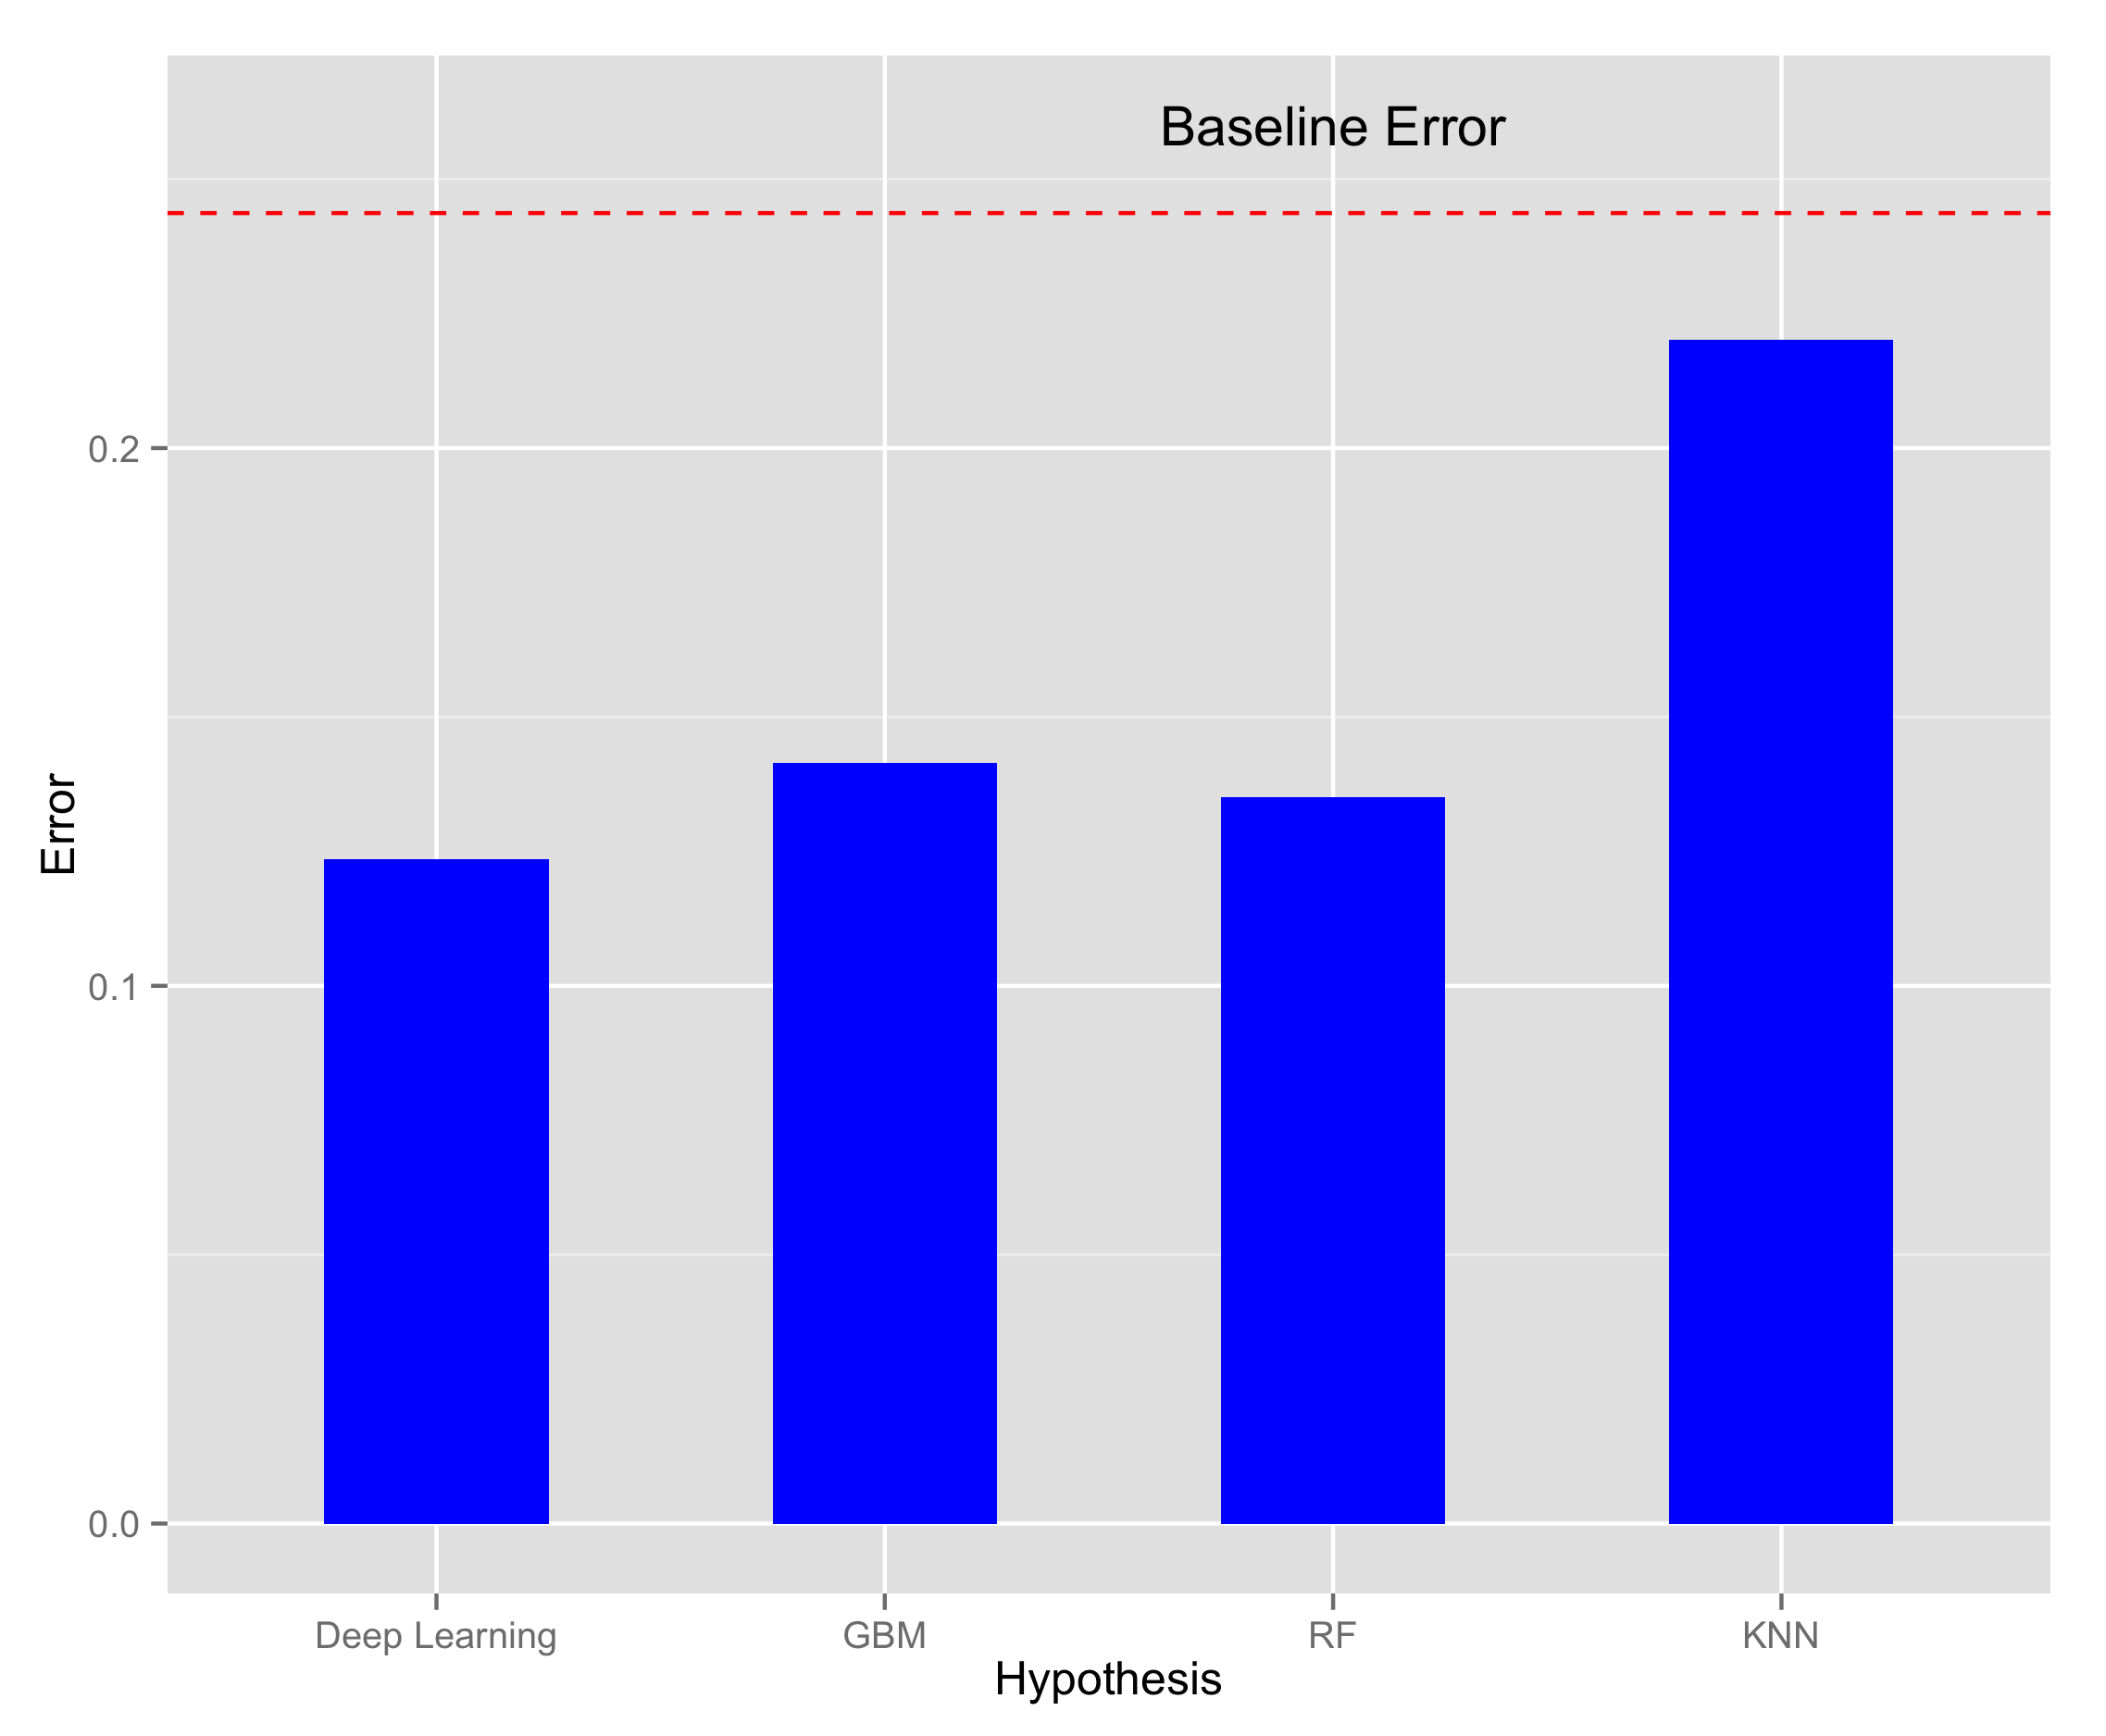
\includegraphics[width=0.8\textwidth]{barchart_initial_errors.png}
    \caption{Initial errors}
    \label{fig:errors}
\end{figure}


We clearly see that the performance of k-NN, at least in the tried configuration with this set of features is rather disappointing. Tree based methods  and neural nets however, show - with some parameter tuning - a significant improvement over the baseline. 


 % % % % % % % % % % % % % % % % % % % % % % % % % % % % % % % % % % % %


\section{Feature Engineering and Model Tuning}

\subsection{Feature Learning}
We settle on Deep Learning and Random Forests, since those performed best in the initial series of experiments. Based on our exploratory analysis, we add several new features to the data set. We feed these into the our previously best performing models, which leaves us with a gain in accuracy. 
Since Deep Learning seems to perform well for this data set, we try a heuristic: Why not train the Random Forest on features extracted with Deep Learning? The recent success on Deep Learning seems to be partly based on it's ability to abstract high-level concepts from the data. For this reason, Machine Learning researchers use it for feature, or representation learning. Feature learning can be done in a supervised or unsupervised manner. We use it in a supervised manner based on the heuristic: the neural net with the highest accuracy will provide the best features for our random forest. Operatively, what is done is just that the nodes of the last hidden layer in the neural net are extracted and used to transform the original feature space. The following figure shows the accuracy of all methods described: Random Forests, Deep Learning, and Random Forests with "Deep Features". 

\begin{figure}[H]
    \centering
    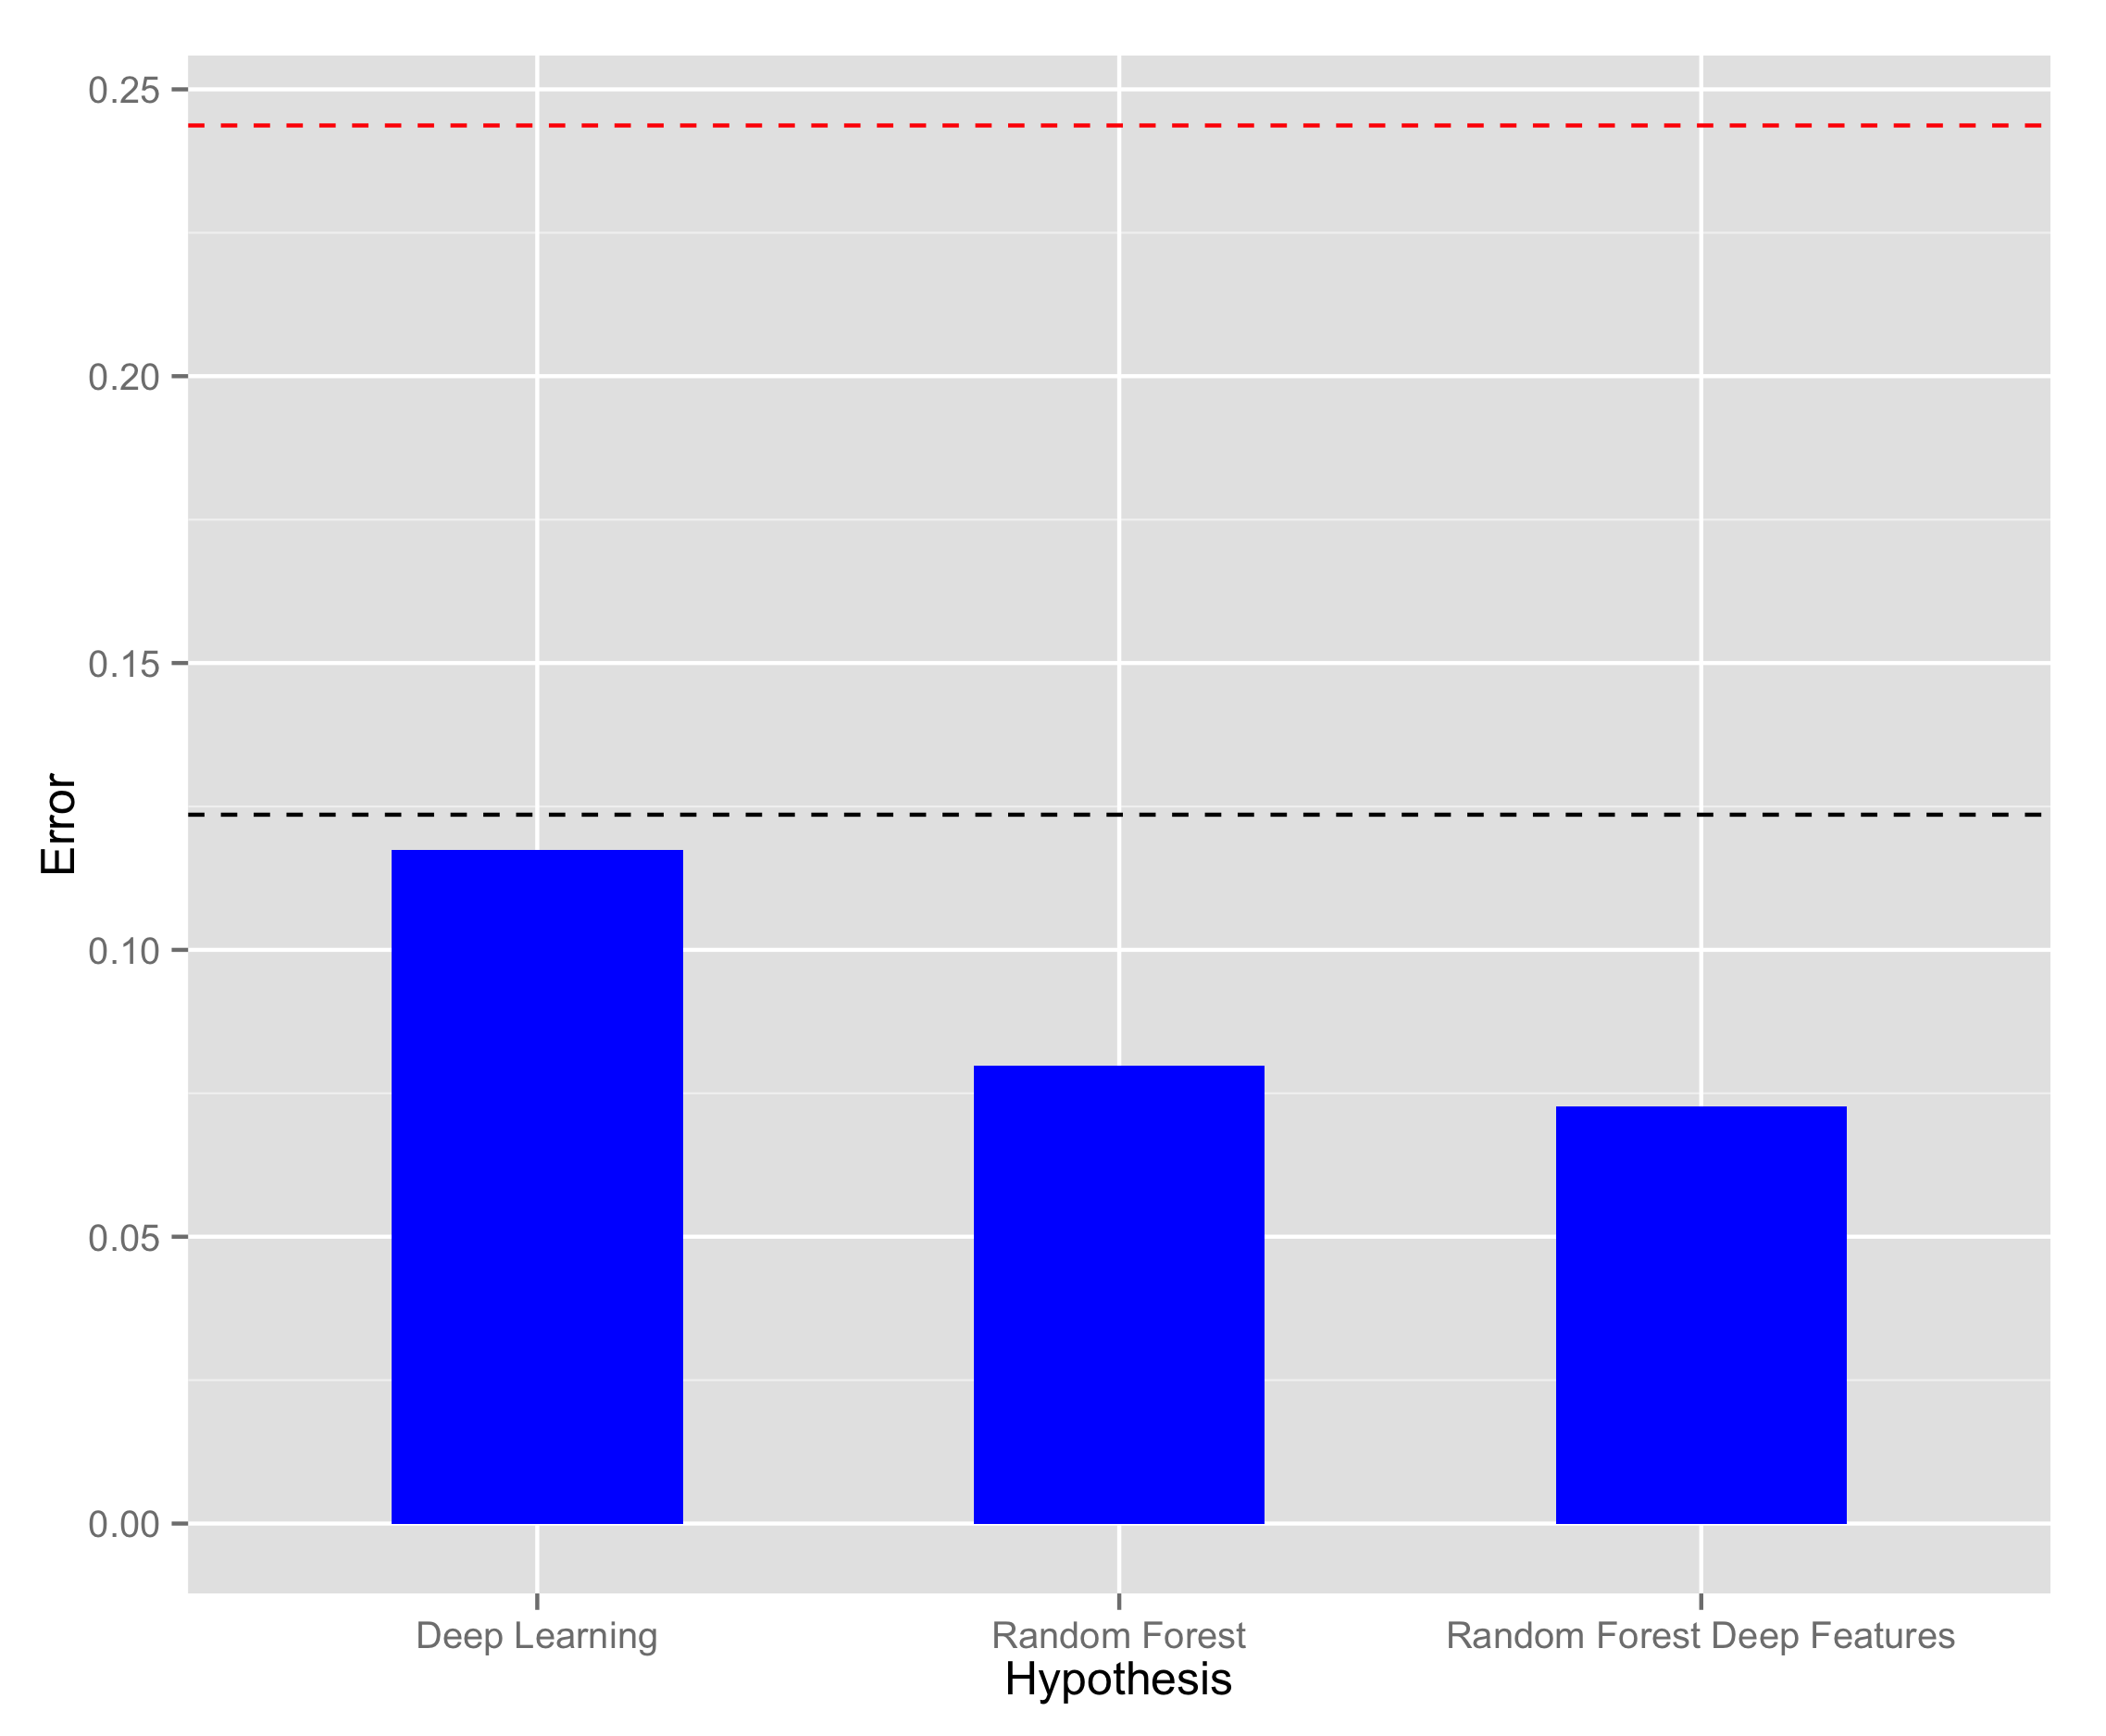
\includegraphics[width=0.8\textwidth]{barchart_new_features_errors.png}
    \caption{Errors with new Features}
    \label{fig:errors}
\end{figure}

We see that this results in a significant gain in accuracy. Apparently, Deep Learning is able to extract useful features from the data. However, in our last example we trained the random forest on 200 features. Too many features may potentially cause overfitting. This is why, in the next series of experiments, we add another layer to the neural net, where the size of the last hidden layer is significantly reduced, thus enforcing sparseness in the output. We try this with 50, 30 and 20 neurons. 

\begin{figure}[H]
    \centering
    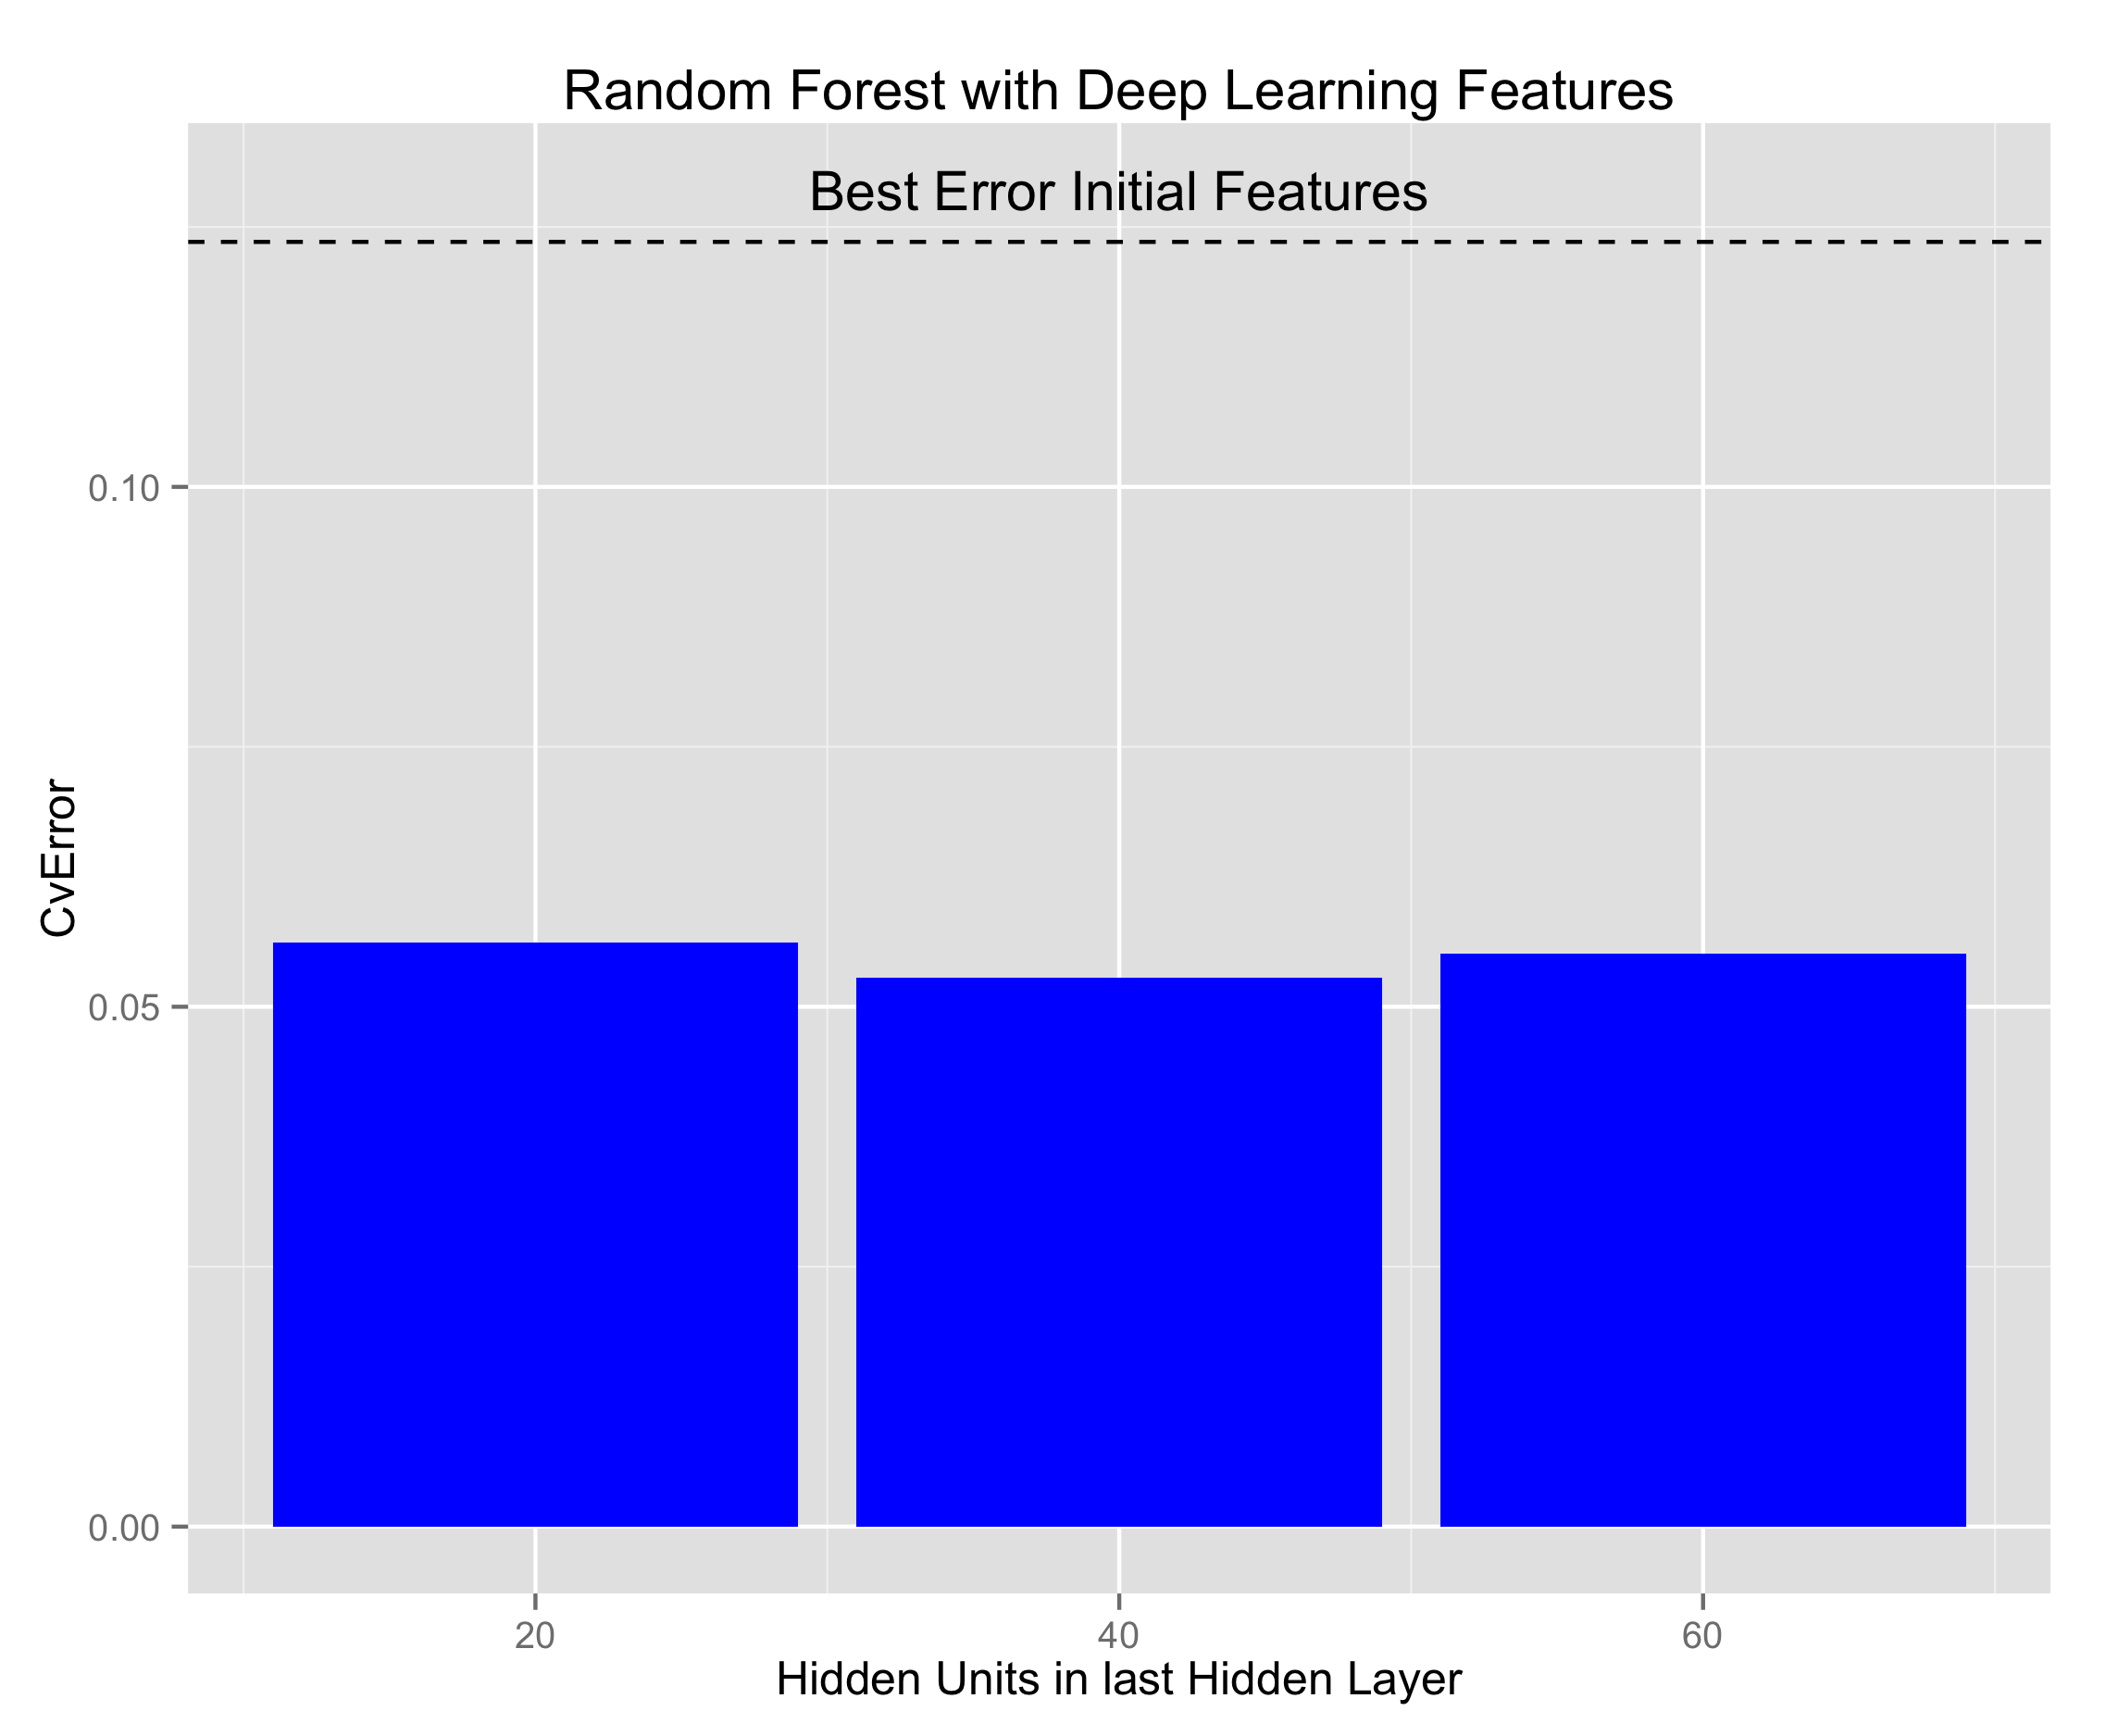
\includegraphics[width=0.8\textwidth]{barchart_error_neurons.png}
    \caption{ Errors of Random Forest with Deep Learning Features }
    \label{fig:errors}
\end{figure}

Here we see, that we are able to again significantly reduce the error of the random forest. 

Now we submit the models with 40 and 60 features for testing. Unfortunately, the test set error is significantly higher: namely we obtain an error of about 0.0965 for each method.
There could be several reasons for this. First, the public leaderboard shows only a 10 percent portion of the actual test data. Second, and more likely is that we overfit: since the cross validation procedure is also only based on the training portion of the data, we might have captured it's structure too well. In fact, a highly complex method, like chaining deep learning and random forests could easily overfit. Therefore, we go back to random forests only and try to find a model that brings our cross validation error close to our training error. 

\subsection{Recursive Feature Elimination}

Random Forests are able to give an estimate of the feature importances. We exploit this fact to use the random forest as a feature selection procedure. The procedure works as follows: We train a random forest and cross validate it. 
We compute the feature importances and the cross validation error. In the next iteration, we leave out the two least important features, and repeat the procedure, recording the CV-Error and the corresponding set of features each time. 
In the following graph, we see the results of said procedure.

\begin{figure}[H]
    \centering
    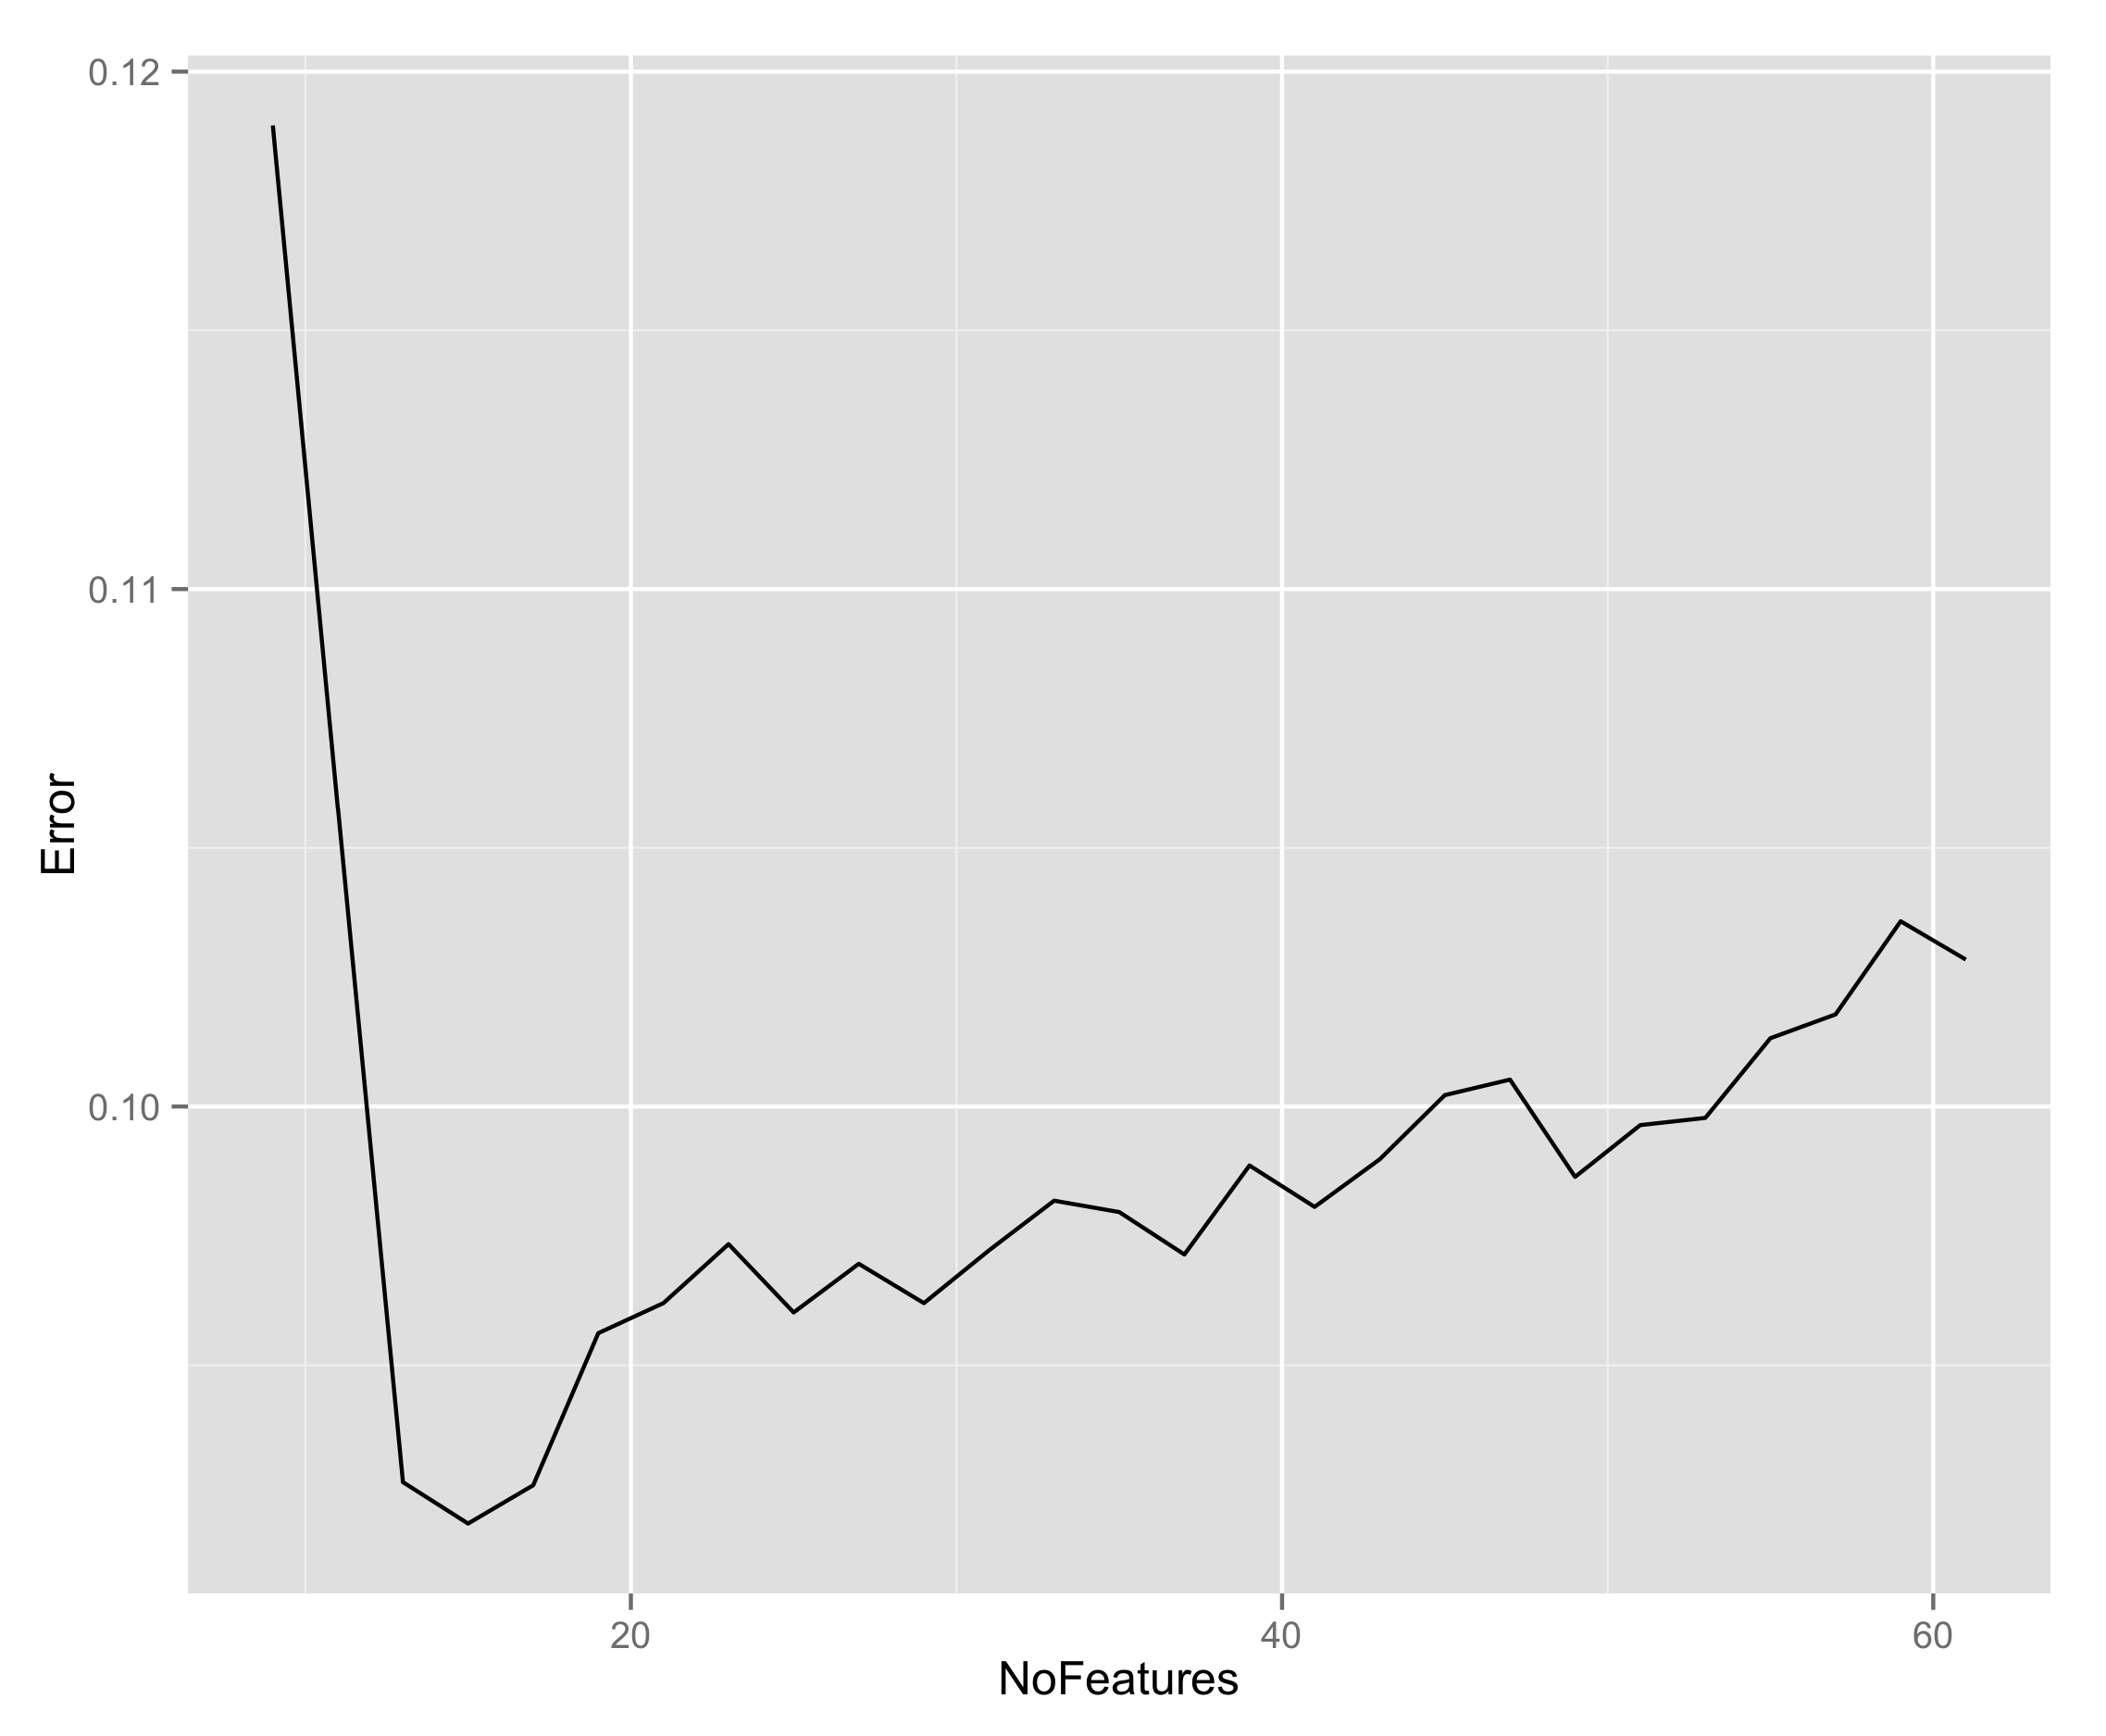
\includegraphics[width=0.8\textwidth]{linechart_results_rfe.png}
    \caption{ Errors of Random Forest with Deep Learning Features }
    \label{fig:errors}
\end{figure}

We see that leaving unnecessary features out can improve generalization performance of our classifier quite significantly. However, leaving out to many features increases the error again.
We choose the best 15, 17, and 29 features (since these have a very low CV-Error), and see if we can tune the parameters further. We increase the fraction used at each iteration of the random forest, since this has been reported to increase accuracy on this dataset, to 0.95. We consider different values (20, 40 and 100) for the maximum depth each single tree has to be grown, where 40 and 100 perform equally well on each set of features. 
The following figure summarizes the errors for the best specification of the random forest algorithm on each subset. 

\begin{figure}[H]
    \centering
    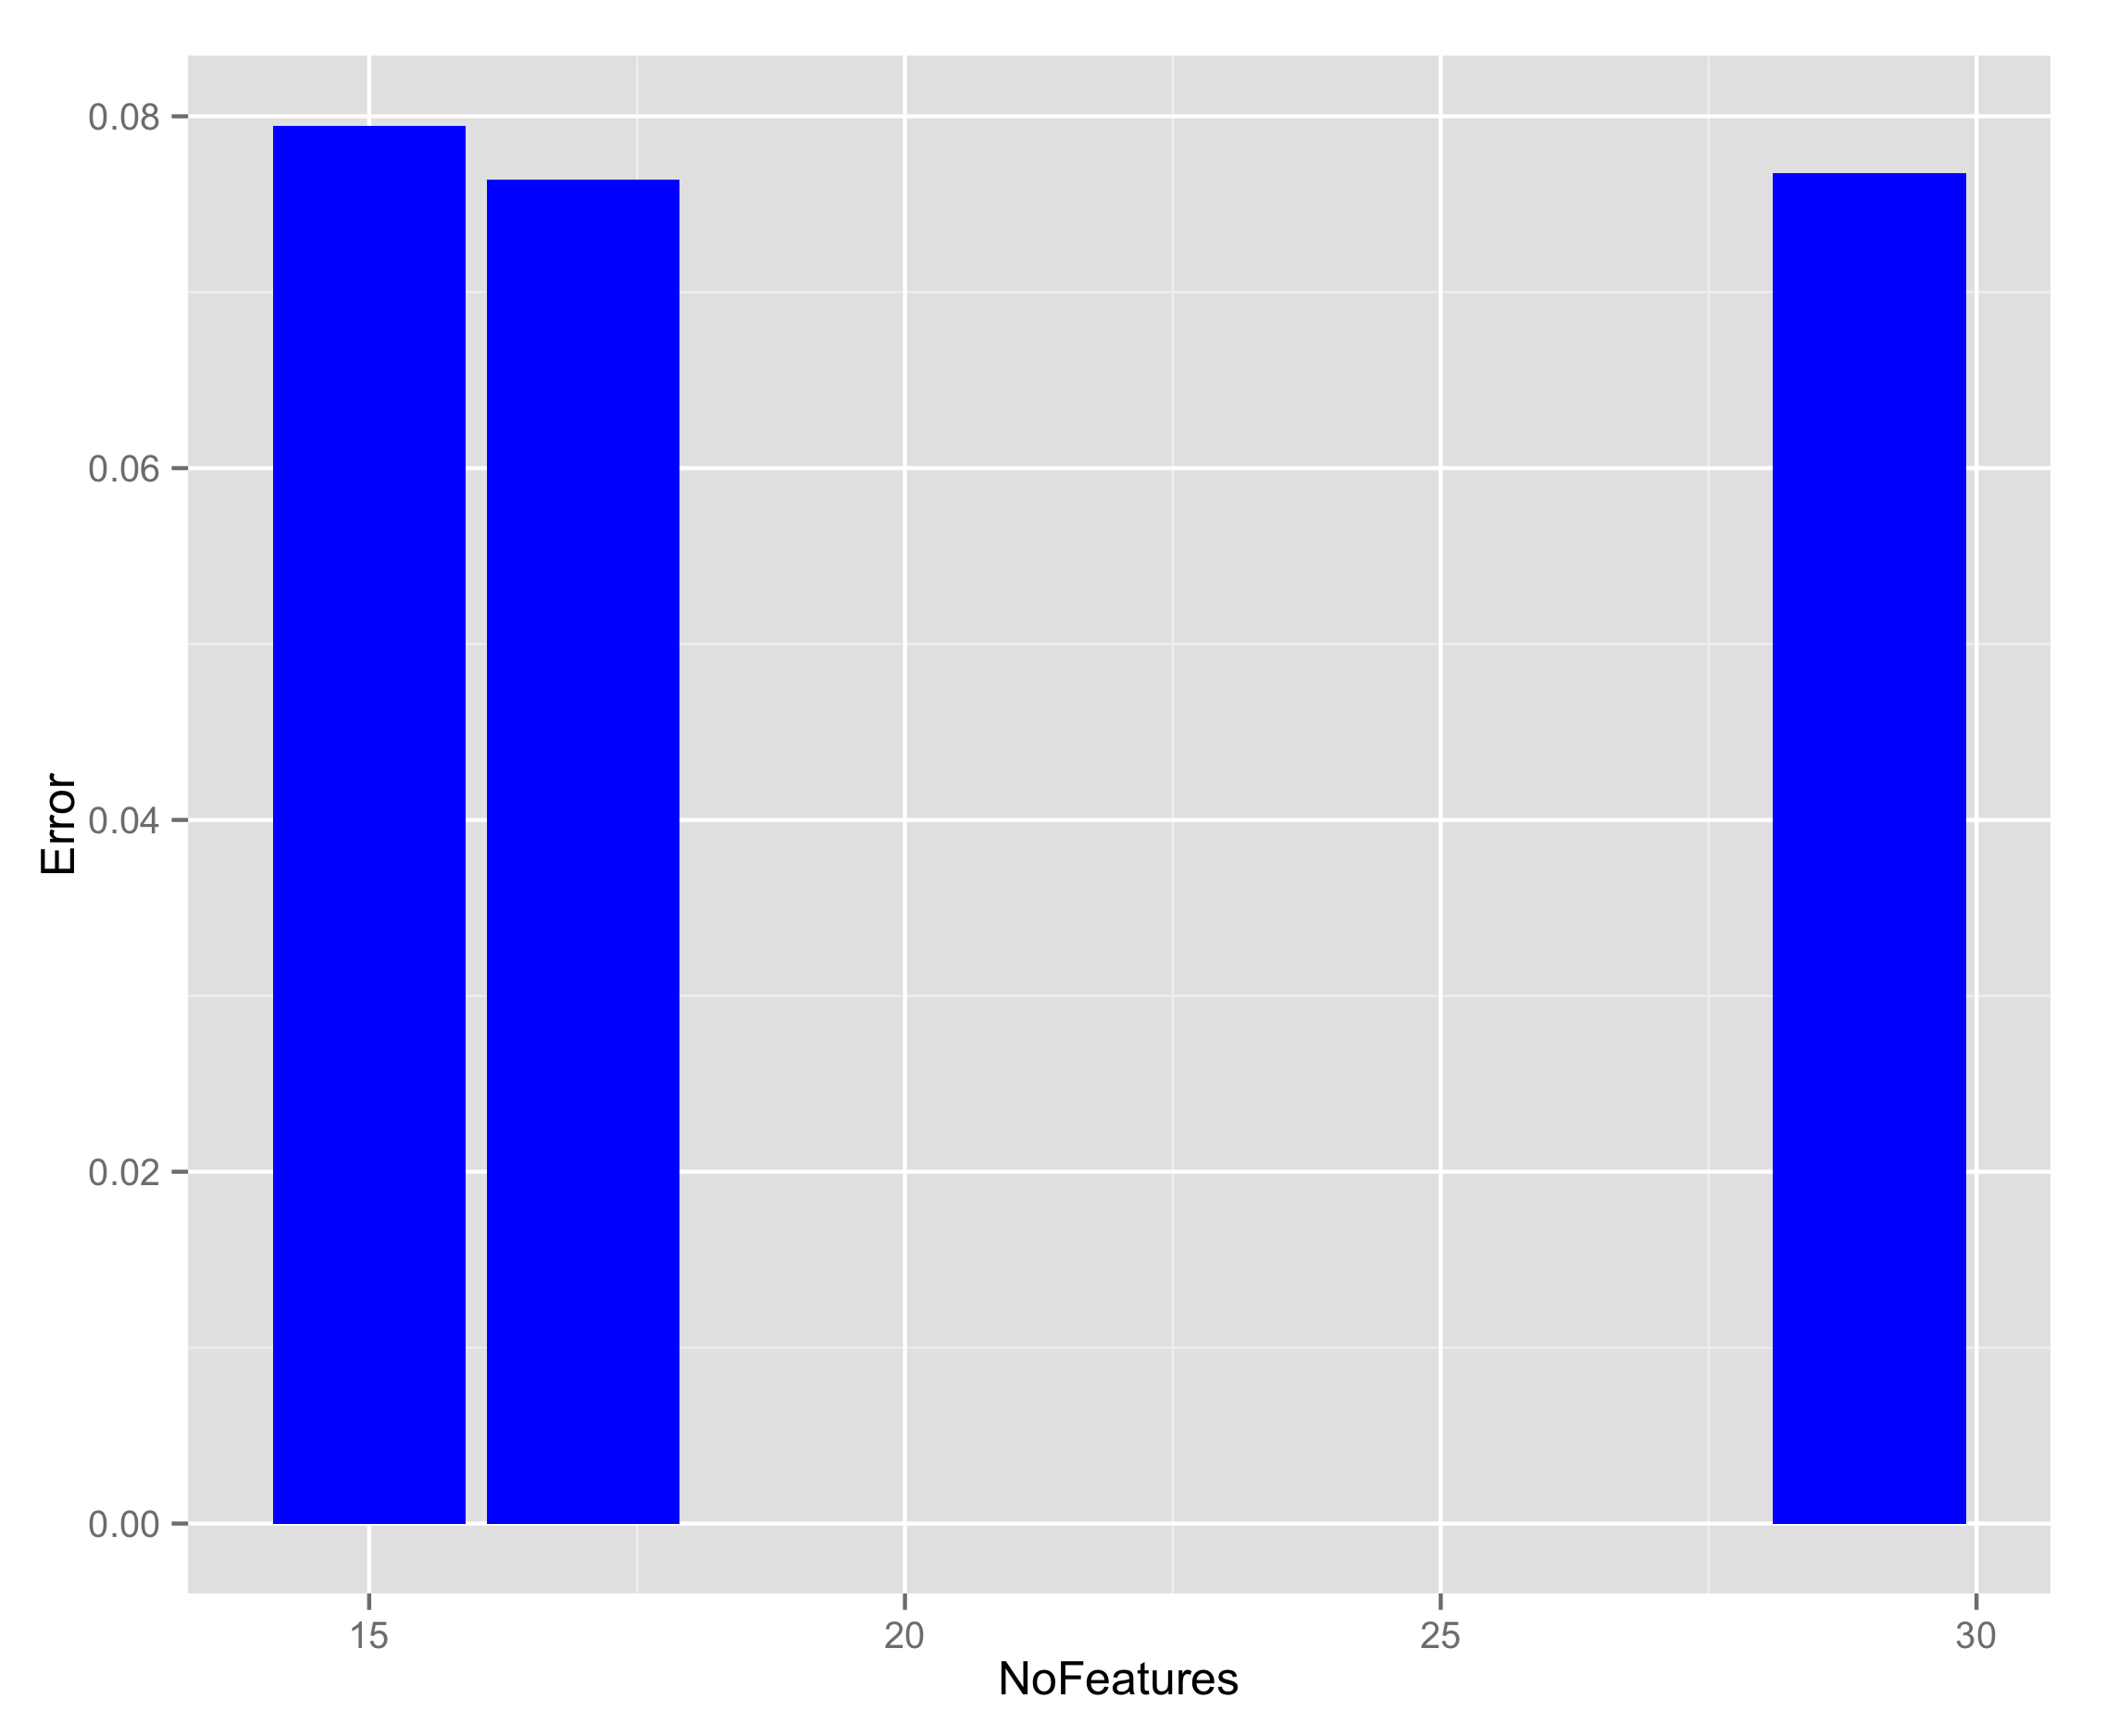
\includegraphics[width=0.8\textwidth]{barchart_best_features.png}
    \caption{ Errors of Random Forest with Deep Learning Features }
    \label{fig:errors}
\end{figure}


We see that 17 features perform best. We try to increase the sample rate parameter which gives us a further improvement (to 0.075). Now we retrain on the full dataset and make predictions on the test set. The resulting submission scores 0.9319, which corresponds to an error of 0.0681. Since the test and and validation error are close in this case, and this model is our best in cross validation (apart from the apparently overfitting models built with deep learning), we decide to opt for this model as our final model. We think that it works best, because utilizes a well known method, and focuses on it's execution. 


 % % % % % % % % % % % % % % % % % % % % % % % % % % % % % % % % % % % %


\section{Limitations}

Some of the main limitations in this project are, firstly, the computational power that we used although we had only a small dataset. 
The extensive use of grid searches required us to use Amazon Web Service (AWS) in order to speed up our calculations. \\ 
Also, our random forest based approach remains largely a black box - although feature importances are computable, it doesn't achieve the explanatory power of, for instance, a logistic regression. 
Finally, it might be possible that we have slightly overfitted jointly the cross-validation and  the visibile test set.

\section{Conclusion}

We predicted the forest cover type with great accuracy using random forests. This leads us to several conclusions. First, as it is well known in the machine learning community, feature engineering is the key to success. Including our own features beyond those that were initially present in the data set, gave us significant accuracy improvements. Second, feature selection: a significant gain in accuracy was achieved by selecting only relevant features. Those made up only one third of the variables. Selecting only relevant features reduces noise in the data and can to a certain extent prevent overfitting. But, since it is carried out - obviously - on the training data, it poses a risk of overfitting in itself. 
Last, once again, the power of ensemble methods was proved. 


 % % % % % % % % % % % % % % % % % % % % % % % % % % % % % % % % % % % %


 % % % % % % % % % % % % % % % % % % % % % % % % % % % % % % % % % % % %

\bibliography{randombib.bib}
	\bibliographystyle{plain}


\end{document}
 % % % % % % % % % % % % % % % % % % % % % % % % % % % % % % % % % % % %
 % % % % % % % % % % % % % % % % % % % % % % % % % % % % % % % % % % % %
 % % % % % % % % % % % % % % % % % % % % % % % % % % % % % % % % % % % %
